\documentclass{article}

\usepackage{tikz}
\usetikzlibrary{calc}
\usepackage[dvipsnames]{xcolor}
\usetikzlibrary{positioning}

\usepackage{Sweave}
\begin{document}
\Sconcordance{concordance:jogo_extensivo1.tex:jogo_extensivo1.Rnw:1 7 1 1 0 19 1}

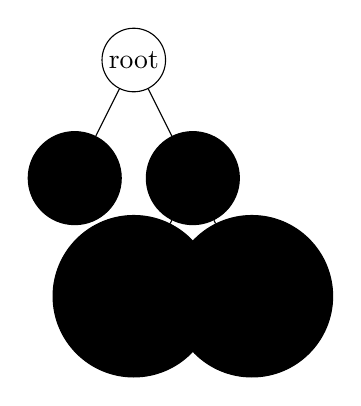
\begin{tikzpicture}
  \tikzstyle{hollow node}=[circle,draw,inner sep=1.5]
  \tikzstyle{solid node}=[circle,draw,inner sep=1.5,fill=black]
  \tikzset{
red node/.style={circle,draw=red,fill=red,inner sep=1.2},
blue node/.style={rectangle,draw=blue,inner sep=2.5}
}
  \node[hollow node](0){root}
  child{node[solid node]{child 1}}
  child{node[solid node]{child 2}
  child{node[solid node]{grandchild 1}}
  child{node[solid node]{grandchild 2}}
  };
\end{tikzpicture}



\end{document}
